%% abtex2-modelo-trabalho-academico.tex, v-1.9.2 laurocesar

%% Copyright 2012-2014 by abnTeX2 group at http://abntex2.googlecode.com/ 
%%
%% This work may be distributed and/or modified under the
%% conditions of the LaTeX Project Public License, either version 1.3
%% of this license or (at your option) any later version.
%% The latest version of this license is in
%%   http://www.latex-project.org/lppl.txt
%% and version 1.3 or later is part of all distributions of LaTeX
%% version 2005/12/01 or later.
%%
%% This work has the LPPL maintenance status `maintained'.
%% 
%% The Current Maintainer of this work is the abnTeX2 team, led
%% by Lauro César Araujo. Further information are available on 
%% http://abntex2.googlecode.com/
%%
%% This work consists of the files abntex2-modelo-trabalho-academico.tex,
%% abntex2-modelo-include-comandos and abntex2-modelo-references.bib
%%

% ------------------------------------------------------------------------
% ------------------------------------------------------------------------
% abnTeX2: Modelo de Trabalho Academico (tese de doutorado, dissertacao de
% mestrado e trabalhos monograficos em geral) em conformidade com 
% ABNT NBR 14724:2011: Informacao e documentacao - Trabalhos academicos -
% Apresentacao
% ------------------------------------------------------------------------
% ------------------------------------------------------------------------

\documentclass[
	% -- opções da classe memoir --
	12pt,				% tamanho da fonte
	openright,			% capítulos começam em pág ímpar (insere página vazia caso preciso)
	twoside,			% para impressão em verso e anverso. Oposto a oneside
	a4paper,			% tamanho do papel. 
	% -- opções da classe abntex2 --
	%chapter=TITLE,		% títulos de capítulos convertidos em letras maiúsculas
	%section=TITLE,		% títulos de seções convertidos em letras maiúsculas
	%subsection=TITLE,	% títulos de subseções convertidos em letras maiúsculas
	%subsubsection=TITLE,% títulos de subsubseções convertidos em letras maiúsculas
	% -- opções do pacote babel --
	english,			% idioma adicional para hifenização
	french,				% idioma adicional para hifenização
	spanish,			% idioma adicional para hifenização
	brazil				% o último idioma é o principal do documento
	]{abntex2}
%https://code.google.com/p/abntex2/wiki/Texmaker
% ---
% Pacotes básicos 
% ---
\usepackage{lmodern}			% Usa a fonte Latin Modern			
\usepackage[T1]{fontenc}		% Selecao de codigos de fonte.
\usepackage[utf8]{inputenc}		% Codificacao do documento (conversão automática dos acentos)
\usepackage{lastpage}			% Usado pela Ficha catalográfica
\usepackage{indentfirst}		% Indenta o primeiro parágrafo de cada seção.
\usepackage{color}				% Controle das cores
\usepackage{graphicx}			% Inclusão de gráficos
\usepackage{microtype} 			% para melhorias de justificação
\usepackage{url}
\usepackage[table,xcdraw]{xcolor}

% ---
		
% ---
% Pacotes adicionais, usados apenas no âmbito do Modelo Canônico do abnteX2
% ---
\usepackage{lipsum}				% para geração de dummy text
% ---

% ---
% Pacotes de citações
% ---
\usepackage[brazilian,hyperpageref]{backref}	 % Paginas com as citações na bibl
\usepackage[alf]{abntex2cite}	% Citações padrão ABNT

%%%%%%%%%%% syntax highlight %%%%%%%%%%%%%%%%%%%%%%%%%%%%%%%%%%%%%%%%%%%%%%%%%%%%%


\usepackage{listings}
\definecolor{maroon}{rgb}{0.5,0,0}
\definecolor{darkgreen}{rgb}{0,0.5,0}
\definecolor{deepblue}{rgb}{0,0,0.5}
\definecolor{deepred}{rgb}{0.6,0,0}
\definecolor{purple}{rgb}{0.5,0,0.5}
\definecolor{deepgreen}{rgb}{0,0.5,0}


 






%%%%%%%%%%%%%%%%%%%%%%%%%%%%%%%%%%%%%%%%%%%%%%%%%%%%%%% 


% --- 
% CONFIGURAÇÕES DE PACOTES
% --- 

% ---
% Configurações do pacote backref
% Usado sem a opção hyperpageref de backref
\renewcommand{\backrefpagesname}{Citado na(s) página(s):~}
% Texto padrão antes do número das páginas
\renewcommand{\backref}{}
% Define os textos da citação
\renewcommand*{\backrefalt}[4]{
	\ifcase #1 %
		Nenhuma citação no texto.%
	\or
		Citado na página #2.%
	\else
		Citado #1 vezes nas páginas #2.%
	\fi}%
% ---

% ---
% Informações de dados para CAPA e FOLHA DE ROSTO
% ---
\titulo{Formalizações analíticas a partir das Teorias dos Conjuntos de Classes de Alturas}
\autor{Guilherme Rafael Soares}
%\local{Brasil}
\data{20 de julho de 2014}
\orientador{Prof. Dr. Daniel Quaranta e Prof. Dr. Alexandre Fenerich}
%\coorientador{Equipe \abnTeX}
\instituicao{%
  UFJF - Universidade Federal de Juiz de Fora
  \par
  Instituto de Artes e Design
  \par
  Programa de Pós-Graduação em Artes, Cultura e Linguagens}
\tipotrabalho{Artigo}
% O preambulo deve conter o tipo do trabalho, o objetivo, 
% o nome da instituição e a área de concentração 
\preambulo{Trabalho final para a disciplina de Análise Musical.}
% ---


% ---
% Configurações de aparência do PDF final

% alterando o aspecto da cor azul
\definecolor{blue}{RGB}{41,5,195}

% informações do PDF
\makeatletter
\hypersetup{
     	%pagebackref=true,
		pdftitle={\@title}, 
		pdfauthor={\@author},
    	pdfsubject={\imprimirpreambulo},
	    pdfcreator={LaTeX with abnTeX2},
		pdfkeywords={abnt}{latex}{abntex}{abntex2}{trabalho acadêmico}, 
		colorlinks=true,       		% false: boxed links; true: colored links
    	linkcolor=blue,          	% color of internal links
    	citecolor=blue,        		% color of links to bibliography
    	filecolor=magenta,      		% color of file links
		urlcolor=blue,
		bookmarksdepth=4
}
\makeatother
% --- 

% --- 
% Espaçamentos entre linhas e parágrafos 
% --- 

% O tamanho do parágrafo é dado por:
\setlength{\parindent}{1.3cm}

% Controle do espaçamento entre um parágrafo e outro:
\setlength{\parskip}{0.2cm}  % tente também \onelineskip

% ---
% compila o indice
% ---
\makeindex
% ---

% ----
% Início do documento
% ----
\begin{document}

% Retira espaço extra obsoleto entre as frases.
\frenchspacing 

% ----------------------------------------------------------
% ELEMENTOS PRÉ-TEXTUAIS
% ----------------------------------------------------------
% \pretextual

% ---
% Capa
% ---
\imprimircapa
% ---

\imprimirfolhaderosto
% ---
% RESUMOS
% ---

% resumo em português
\setlength{\absparsep}{18pt} % ajusta o espaçamento dos parágrafos do resumo
\begin{resumo}


A proposta deste artigo é organizar um estudo computacional da corrente musicológica que trabalha sobre as \textit{teorias dos conjuntos de classes de altura}. Para isso buscamos referenciar taxonomias \cite{forte1973structure}, descrever operações de transformação \cite{straus2004} e problematizar uma análise musical capaz de apontar singularidades em composições \cite{lester1989analytic,straus2004} que não necessariamente operam sobre os pressupostos de uma expectativa de tonalidade explícita do repertório de prática comum.



 \textbf{Palavras-chaves}: Música algorítmica. Pós-tonalismo. Teoria dos conjuntos de classes de altura. Pitch class set theory
\end{resumo}



% ---
% Capitulo de revisão de literatura
% ---


\chapter{Teorias dos Conjuntos das Classes de Alturas }
\label{modelos}

Nas \textit{teorias dos conjuntos de classes de altura} (\textit{"Pitch Class Set Theory"}), os intervalos são tratados de maneira neutra em relação a qualquer centro tonal pré-determinado. Parte-se do princípio de que agrupamentos de alturas podem gerar estruturas de derivadas por uma espécie de parentesco intervalar, incluindo a similaridade por inversão ou retrógrado destes, como veremos mais adiante. 

Essas teorias são fortemente influenciadas pela ideia de serialismo - formalizada pelo dodecafonismo frequentemente atribuído a Arnold Shoenberg e seus seguidores da segunda escola de Vienna. No entanto, é bom lembrar que o pensamento serial é um pensamento composicional que pode também ser encontrado em compositores muito anteriores a estas formalizações\cite{lester1989analytic}. Podemos encontrar tal abordagem analítica sendo usada para destacar aspectos de composições de outros contextos que não o restrito ao repertório atonal clássico. Como faz, por exemplo, Joel \citeonline{lester1989analytic}, em sua didática para análises de um repertório pós-tonal do início do século XX, ou Allen Forte, na sua tese sobre a "Sagração da Primavera"\ de Stravinski \cite{forte1978harmonic}.

\begin{citacao}
Foi, obviamente, Allen Forte quem foi o pioneiro das análises com a taxonomia dos grupos de classes de alturas aplicadas em conceitos da matemática, primeiro surgindo em tipos de Milton Babbit (a teoria conceitual), e em seguida com a inclusão e abstração de relações (como as relações de similaridade) construídas para uso analítico. A \textit{"teoria dos conjuntos de classes de altura}"\ de Forte (...) tem tido suas próprias ramificações e influência. Em particular, as próprias análises de Forte de peças individuais tem levado muitos outros a fazerem de maneira parecida, e a ideia inicial de Forte das relações de similaridade (diferentes das relações de equivalência) sobre os grupos de classes de alturas tem visto florescer uma indústria teórica em torno disto, depois que os artigos seminais de Morris, Rahn  Lewin apareceram em 1980. \cite[ p. 130]{rahn2004swerve}\footnote{
It was, of course, Allen Forte who in the USA pioneered the analytical with a taxonomy of pc-set application of concepts from mathematics, first arose also in serial Babbittian types (the concept theory), and following as some inclusion and with relations abstract up (such similarity relations) meant for analytical use. Forte's "set theory"\  (...) has had its own ramifications and influence. In particular, Forte's own analyses of individual pieces of music have led many others to do likewise, and Forte's initial idea of similarity relations (as distinct from equivalence relations) among pitch-class sets has seen a flourishing theoretical industry grow around it, after seminal articles by Morris, Rahn, and Lewin appeared in 1980. \cite[ p. 130]{rahn2004swerve}}
\end{citacao}




Com a formalização das \textit{teorias dos conjuntos de classes de alturas} pela geração de musicólogos e compositores seriais da segunda metade do século XX, e com os avanços exponenciais da computação nas últimas décadas, estas teorias vão sendo testadas e aplicadas a ponto de já constituírem uma área bastante específica da musicologia contemporânea \cite{aroundset2013}.

Um exemplo de interesse do presente trabalho é a classe de objetos "Math Tools"\ \cite{andreatta2003implementing,AndreataOMtutorial,DebrilOM} da linguagem de programação OpenMusic\footnote{c.f. \url{http://repmus.ircam.fr/openmusic/home}}, que organiza em orientação a objetos uma série de conceitos que veremos logo a seguir. 



\section{Fórmulas de agrupamento e transformação dos intervalos}

A teoria dos conjuntos de classe de altura utiliza como base de suas formulações a relação entre os 12 semitons da escala cromática de forma modular. Consideram-se neste sentido alturas de mesma oitava como sujeitas mesmas propriedades intervalares, podendo argumentar relações independentes de registro. Exemplo: o Dó grave - representado no protocolo MIDI pelo valor 24 - tem uma relação de equivalência com o Dó agudo de valor 72. A fórmula é simples: ambos, quando divididos por 12, apresentam resto 0. A nota Ré, por exemplo, sempre apresenta o resto 2, e assim por diante. Dizemos por tanto que pertencem a uma mesma classe de altura.

Diferente de quando argumentada uma "enarmonia funcional" \cite{temperley2001cognition} (como por exemplo D\# $\to$ Eb), a teoria dos conjuntos das classes de altura não toma como princípio ideias do tipo "terça maior ou menor", "nota sensível" ou "nota de passagem"\ pois vai partir de uma relação direta entre aglomerados sonoros, buscando similaridades e equivalências sem estar tão presa a formas de prolongamento normatizadas pelo tonalismo clássico \cite{lerdahl1989atonal,straus1987problem}.

Os intervalos são, sobretudo, distâncias. Nas \textit{teorias dos conjuntos de classes de alturas} essas distâncias podem estar categorizadas como intervalos ordenados - usando número negativos para os intervalos descendentes, ou não-ordenados - considerando intervalos equivalentes independentes de suas direções \cite[p. 6]{straus2004} Isso cria imediatamente uma relação interessante de parentesco entre pares em todos intervalos da escala cromática - exceto para o trítono, intervalo de sexta ordem que está equidistante de 0 e 12 e portanto não possui uma inversão propriamente dita, mas sim tem o papel de cortar ao meio este espelhamento.

\begin{figure}[!h]
	\caption{\label{fig_grafico}Equivalência de intervalos por inversão }
	\begin{center}
	    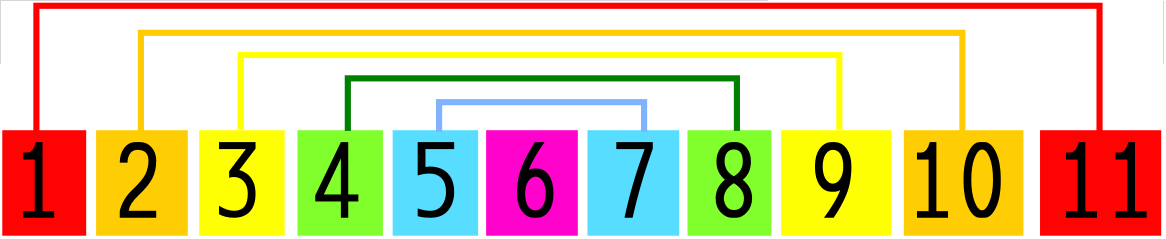
\includegraphics[scale=0.3]{algo/equivalencia_inversa.png}
	\end{center}
	\legend{Fonte: autor }
\end{figure}




\subsection{Vetor intervalar}

A operação de obtenção do vetor intervalar é a primeira das reduções sugeridas para propor uma similaridade entre agrupamentos que seja neutra quanto a inversões e oitavas.

Tomemos um exemplo de uma sequência C-D-E-Bb.



\begin{figure}[!h]
	\caption{\label{fig_grafico}[0,2,4,10] }
	\begin{center}
	    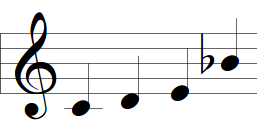
\includegraphics[scale=0.6]{OM_settheory/vetor02410.png}
	\end{center}
	\legend{Fonte: autor }
\end{figure}


Este trecho pode ser reduzido a sequência de alturas [0,2,4,10]

Organizamos seus intervalos fazendo todas as combinações possíveis entre essas distâncias:


$ inversões = \left\{
  \begin{array}{l l}
    2-0 = 2\\
    4-0 = 4\\
    10-0 = 10 \\
     \\
    4-2 = 2\\
    10-2= 8 \\
     \\
    10-4= 6
  \end{array} \right.
$

O vetor de intervalos pode ser reduzido então a uma contagem que coloca no mesmo grupo os intervalos que são inversões dos primeiros cinco intervalos possíveis, já que seus pares após o trítono não são considerados espelhamentos. No exemplo acima temos 10 que é a inversão de 2, e 8 que é a inversão de 4. Nosso vetor fica assim:


\begin{table}[h]
\begin{tabular}{|
>{\columncolor[HTML]{FD6864}}l |
>{\columncolor[HTML]{F8A102}}l |
>{\columncolor[HTML]{F8FF00}}l |
>{\columncolor[HTML]{34FF34}}l |
>{\columncolor[HTML]{00D2CB}}l |
>{\columncolor[HTML]{EE00EE}}l |}
\hline
1 & 2 & 3 & 4 & 5 & 6 \\ \hline
0 & 3 & 0 & 2 & 0 & 1 \\ \hline
\end{tabular}
\end{table}

Pode-se dizer então que a classe de alturas [0,2,4,10] possui o vetor intervalar <0,3,0,2,0,1>.


\subsection{Forma Normal} 

É comum na prática dos grupos de classes de altura a preparação dos conjuntos em sua forma ordenada e reduzida. Desta maneira podemos mais facilmente reconhecer as equivalências entre os grupos, reconhecer transposições, propriedades.


\begin{figure}[h]
	\caption{\label{fig_grafico}Redução de um segmento do Microkosmos 101 de Bartók para um \textit{cluster} de 4 alturas. }
	\begin{center}
	    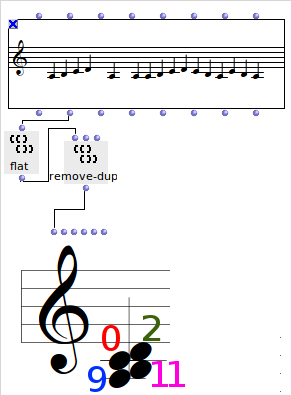
\includegraphics[scale=0.7]{OM_settheory/reducao_acorde.png}
	\end{center}
	\legend{Fonte: autor }
\end{figure}

Para a redução de uma forma normal, partimos do \textit{cluster} sem repetições, colocando todas as alturas dentro da mesma oitava. Os passos seguintes são: 
\textbf{a)} Ordenar de forma ascendente e escolher a sequência que tenha a menor distância da primeira até a última nota.
\textbf{b)} Se houver empate, reduzir pela que seja mais compacta à esquerda, comparando o menor intervalo entre a primeira e penúltima e assim por diante.
\textbf{c)} Havendo ainda empate, escolher aquele grupo que tem a menor altura como início. 

\begin{figure}[h]
	\caption{\label{fig_grafico}Forma Normal. }
	\begin{center}
	    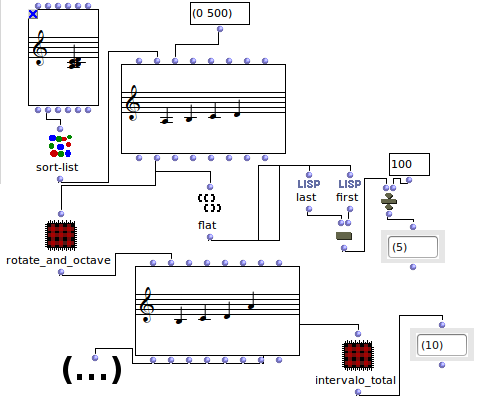
\includegraphics[scale=0.7]{OM_settheory/forma_normal.png}
	\end{center}
	\legend{Fonte: autor }
\end{figure}



\pagebreak
\subsection{Forma Prima} 

A forma prima é um procedimento para simplificar ainda mais a forma normal, encontrando "a mais normal das normais"\ \cite[p. 47]{straus2004} e reduzindo vetores que possuem os mesmos intervalos ou são inversões e transposições a um vetor primário. Para isso uma forma normal é transposta até que possua o zero em sua primeira posição. O mesmo é feito com sua inversão. A forma mais compacta à esquerda será a forma prima. Allen \citeonline{forte1973structure} desenvolveu uma taxonomia a partir das formas primas que tem sido utilizada como forma canônica para representação de grupos de classes de altura.\footnote{A biblioteca \textit{"math"}\ do OpenMusic possui o objeto "p-form"\ para encontrar os agrupamentos de Forte. A tabela original está no livro "The Structure of Atonal Music"\ \cite[p.179-181]{forte1973structure}}. Forte organiza agrupamentos pelo número de elementos seguidos por um número que diz a ordem dentro de um conjunto com aquele mesmo número de elementos. Exemplo: |3-1| é composto das alturas (0,1,2), |3-2|  é o \textit{cluster} (0,1,3), |4-17|  é composto por (0,3,4,7), e assim por diante.

\begin{figure}[h]
	\caption{\label{fig_grafico}Fórmulas de agrupamento de classes de altura. }
	\begin{center}
	    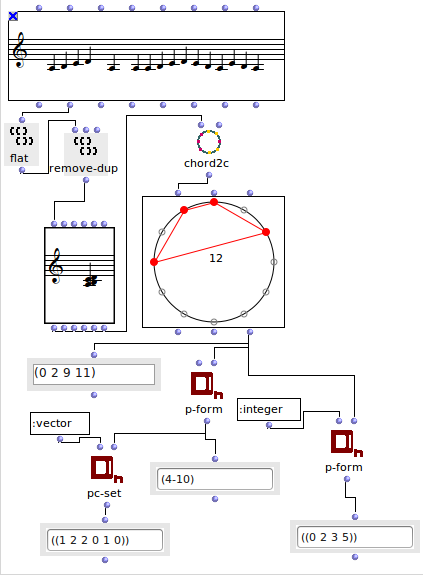
\includegraphics[scale=0.7]{OM_settheory/forma_prima_forte_vector.png}
	\end{center}
	\legend{Fonte: autor }
\end{figure}





%\begin{citacao}
%Two Algorithms for Computing the Prime Form

%There are two algorithms for computing the prime form of a Pitch Class Set. The first was introduced by Allen Forte %in The Structure of Atonal Music and the second is used by John Rahn in his book Basic Atonal Theory and is also %used by Joseph N. Straus in his Introduction to Post-Tonal Theory.

%The difference between the two algorithms is apparent when examining Pitch Class Set 6-31. The Prime Form using the %Forte algorithm is (0,1,3,5,8,9), and the prime form using the Rahn algorithm is (0,1,4,5,7,9). As you can see, the %Forte algorithm puts a priority on making the small numbers smaller (i.e. 3 instead of 4), whereas the Rahn %algorithm wants the larger numbers to be smaller (i.e. 7 instead of 8).

%Which is better? Well, it depends on who you ask. Computer programmers and computer music people will typically %prefer the Rahn algorithm because it is computationally more elegant. However, the Forte algorithm has the more %established pedigree, and so it tends to be preferred by academics.

%Fortunately, this is usually a minor issue because it only affects the following 5 sets:

%Pitch Class Set	Forte Prime	Rahn Prime
%5-20	(0,1,3,7,8)	(0,1,5,6,8)
%6-Z29	(0,1,3,6,8,9)	(0,2,3,6,7,9)
%6-31	(0,1,3,5,8,9)	(0,1,4,5,7,9)
%7-20	(0,1,2,4,7,8,9)	(0,1,2,5,6,7,9)
%8-26	(0,1,2,4,5,7,9,10)	(0,1,3,4,5,7,8,10)
%\end{citacao}


\subsection{Singularidades nos agrupamentos }

Algumas propriedades entre os grupos de classes de alturas são muito interessantes como princípio composicional e, mesmo quando não sendo tão óbvias em primeiras audições, contribuem ao menos com uma coerência estrutural e conceitual. George Perle argumenta sobre "funções motívicas"\ em grupos de alturas \cite [p. 60-85]{perle1991serial} e observa algumas estratégias de compositores para aproveitar algumas propriedades encontradas em relações internas das séries. Perle no entanto mostra-se cético quanto a formalização de nomenclaturas analíticas derivadas da classificação de Allen Forte e questiona sua aplicação em argumentações para análises de composições que tenham sido compostas antes das fórmulas tornarem-se ferramentas musicológicas. \cite{perle1990pitch}

Levantaremos aqui algumas destas propriedades conforme o resumo didático proposto por \citeonline{straus2004}, sem ainda estarmos certos de sua efetividade para análises, pelo interesse em uma possível formalização computacional destas propriedades para processos composicionais.


\subsubsection{Notas comuns sob transposição}

Tomemos o seguinte exemplo: Dado um grupo em sua forma prima [0,2,5] - ou "4-10"\ na forma prima pela classificação de Allen \citeonline{forte1973structure} - quando transpomos para o intervalo 2 e seu inverso 10, obtemos duas notas iguais para cada um destes grupos.

\begin{figure}[!h]
	\caption{\label{fig_grafico}Notas comuns na transposição. }
	\begin{center}
	    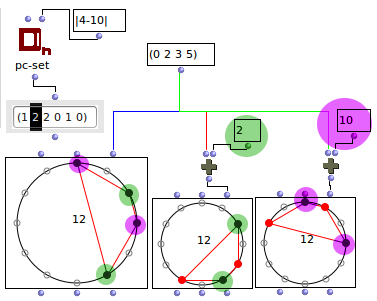
\includegraphics[scale=0.7]{OM_settheory/notas_comuns_2e10.png}
	\end{center}
	\legend{Fonte: autor }
\end{figure}



Isso acontece porque o vetor de intervalos para esta forma é <1,2,2,0,1,0>, e podemos observar que há uma fórmula geral que prova que o número de incidências comuns de uma determinada classe de alturas em sua transposição será o número de repetições deste intervalo em seu vetor original. Neste caso por exemplo temos duas incidências do intervalo de classe 2, e portanto as transposições T2 e T10 têm duas notas em comum com T0.

Há uma exceção a esta regra:
 
\begin{figure}[!h]
	\caption{\label{fig_grafico}Notas comuns na transposição com trítono. }
	\begin{center}
	    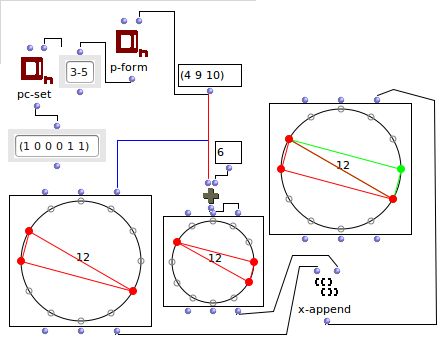
\includegraphics[scale=0.7]{OM_settheory/notas_comuns_tritono.png}
	\end{center}
	\legend{Fonte: autor }
\end{figure}

É preciso observar que para o caso do trítono a inversão é simétrica - portanto para cada trítono temos duas notas em comum. Como no exemplo acima: 10 e 4 geram as duas simétricas 4 e 10, logo conclui-se que um trítono gera duas notas em comum e assim por diante.

Interessante pensar também que o vetor de intervalos irá determinar transposições onde não existe nota nenhuma em comum. Composicionalmente isso pode ser visto como uma possibilidade de transpor a série para uma sessão totalmente distinta da anterior, criando algum discurso com estas transições.


\subsubsection{Simetria Transpositiva}

Na simetria transpositiva temos um padrão de intervalos que funciona como palíndromo (tem a mesma leitura da esquerda para a direita e direita para esquerda).

\begin{figure}[!h]
	\caption{\label{fig_grafico}A simetria transpositiva é obtida através de um padrão de intervalo palíndromo. }
	\begin{center}
	    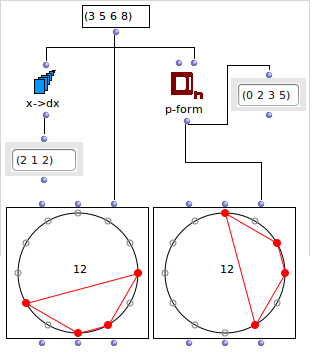
\includegraphics[scale=0.6]{OM_settheory/palindrome1.png}
	\end{center}
	\legend{Fonte: autor }
\end{figure}



\begin{figure}[!h]
	\caption{\label{fig_grafico}A forma circular é mais geral do que a numérica para a visualização do padrão de simetrias. }
	\begin{center}
	    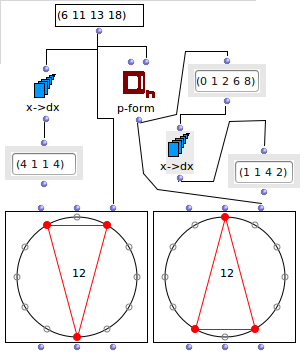
\includegraphics[scale=0.6]{OM_settheory/palindrome2.png}
	\end{center}
	\legend{Fonte: autor }
\end{figure}



\subsubsection{Complemento}

Útil para reconhecer e produzir contextos totalmente distintos entre si, o complemento é composto por todos intervalos que estão exclusos dos grupo, produzindo um outro grupo completamente diferente.


\begin{figure}[!h]
	\caption{\label{fig_grafico}O complemento contém todas as alturas cromáticas que o conjunto original não possui. }
	\begin{center}
	    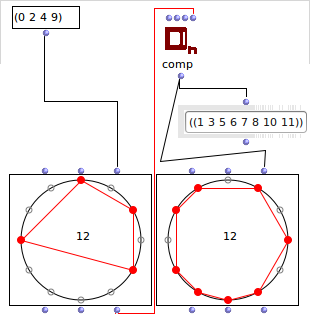
\includegraphics[scale=0.6]{OM_settheory/complemento.png}
	\end{center}
	\legend{Fonte: autor }
\end{figure}


\subsubsection{Relação Z entre grupos de classes de alturas}

A relação Z é uma das interessantes relações onde há uma equivalência sem que os conjuntos sejam transposições ou inversões entre si - neste caso, produzindo dois conjuntos que possuem os mesmos intervalos na sua constituição.


\begin{figure}[!h]
	\caption{\label{fig_grafico}Dois conjuntos Z-relacionados possuem os mesmos intervalos sem serem inversões ou transposições uns dos outros. }
	\begin{center}
	    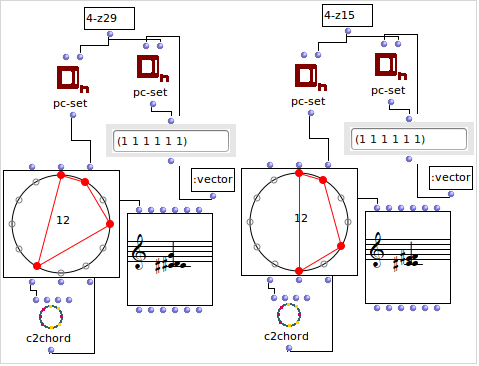
\includegraphics[scale=0.7]{OM_settheory/Z_related.png}
	\end{center}
	\legend{Fonte: autor (adaptado de exemplo do tutorial MathTools do OM) }
\end{figure}


George Perle exemplifica a relação Z como uma das relações que não são intuitivas em sua rotina composicional:

\begin{citacao}
Mas nenhum destes argumentos teria qualquer peso para mim se eu pudesse ao menos escutar as correspondências que Forte descreve. Eu posso descobrir estas conexões entre coleções Z-relacionadas somente sujeitando-as a um escrutínio analítico que não tem nada a ver com minha experiência intuitiva como ouvinte ou compositor. Ou, para falar de maneira mais sincera, permitir que o Professor Forte conduza seu escrutínio analítico para mim.
\cite[ p. 168]{perle1990pitch}\footnote{
But none of these arguments would carry any weight with me if
I could only hear thes correspondences that Forte describes. I can
discover these connections between Z-related collections only by sub-
jecting them to an analytical scrutiny that has nothing whatever to do
with my intuitive experience as a listener or as a composer. Or, to
speak more candidly, by allowing Professor Forte to conduct this
analytical scrutiny for me. 
\cite[p.168]{perle1990pitch}}
\end{citacao}

Perguntamo-nos se este tipo de afirmação não seria um tanto arbitrária. Afinal, as diferenças entre terças maiores e menores não seriam no fundo resultado de uma exposição cultural constante a estes intervalos usados como critério de diferença ou similaridade? Consequentemente a geometria e propriedades transformacionais das terças acabam polarizando o próprio conceito de acorde. Se toda estrutura musical emerge de um condicionamento cultural da escuta, por onde buscar novas escutas?

Parece que de alguma maneira a relação Z acaba por nomear uma sonoridade por uma particularidade entre relação numérica e geométrica curiosa, e no mínimo serve como mnemônico de uma relação entre estas sonoridades.

\subsection{Arbitrariedade e indução  na segmentação atonal}

Encontrar estas relações em composições anteriores a sua formalização é o que \citeonline{nattiez2001tripartite} chama de "estésica indutiva".

Esta questão nos leva a uma inevitável aporia. Há uma série de esforços para comprovar tanto a eficácia quanto a ineficácia desta teoria para aplicação em análises. Um exemplo é a tese de Ethan \citeonline{haimo1996atonality} que busca "falácias"\ no esquema analítico clássico das \textit{teorias dos conjuntos de classes de alturas} quando confrontado com anotações originais de Arnold Shoenberg.

\citeonline{straus2004} sentencia:

\begin{citacao}
A resposta é que você não pode saber com antecedência.
Você tem que entrar no mundo da peça – ouvindo, tocando, e cantando – até que você
obtenha um senso de quais ideias musicais são fundamentais e recorrentes. No processo,
você encontrar-se-á movendo-se em torno de um tipo familiar de círculo conceitual. Você
não pode saber quais são as principais ideias até que você as veja recorrer; mas você não
pode encontrar recorrências até que você saiba quais são as ideias principais. A única
solução prática é bisbilhotar a peça, propondo e testando hipóteses conforme você
prossegue. 
\cite{straus2004}
\end{citacao}

\citeonline{nattiez2003allen} faz uma crítica minuciosa da aplicação das \textit{teorias dos conjuntos de classes de alturas} derivadas do trabalho de Allen Forte, em busca de uma descrição estésica que justifique a aplicação de toda a formalização de seu nível neutro de nomenclaturas e chega à seguinte conclusão:


\begin{citacao}
(...)seria fascinante ver que resultados obteríamos comparando grupos que descreveriam unidades previamente segmentadas por uma análise paradigmática num nível neutro. Se nos sentimos intimidados a confiar nas análises preliminares, com efeito, o caleidoscópio com o qual o analista vai descobrir trabalhos atonais vai efetivamente ser fruto de operações mágicas, não porque o compositor escondeu-as ali, mas porque o musicologista, através do truque com as mãos, esta agindo como um mágico! \cite[ p. 16]{nattiez2003allen}\footnote{(...)it would be fascinating to see what results we would obtain from comparing sets which would describe units previously segmented by a paradigmatic analysis at the neutral level. If we do feel compelled to rely on this preliminary analysis, in effect, the kaleidoscope which the analyst will discover in atonal works will effectively be the fruit of magical operations, not because the composer hid them there, but because the musicologist, through sleight of hand, was acting like a magician!
\cite[ p. 16]{nattiez2003allen}}
\end{citacao}





% ---

% ---
% Conclusão (outro exemplo de capítulo s


% ---

% ---
% Conclusão (outro exemplo de capítulo sem numeração e presente no sumário)
% ---em numeração e presente no sumário)
% ---
\chapter*[Conclusão]{Conclusão}
\addcontentsline{toc}{chapter}{Conclusão}
\label{conclusao}
% ---

Nas últimas décadas do século XX\footnote{A partir da sedimentação de uma tradição pós-tonal iniciada nas primeiras décadas do século XX.} formalizaram-se "\textit{teorias dos conjuntos de classes de alturas}"\cite{forte1973structure,rahn1980basic,perle1990pitch,straus2004} baseadas numa catalogação de combinações de intervalos formando compostos sonoros singulares e as possíveis estruturações e articulações entre estes. Ali operariam critérios não necessariamente tão amarrados na funcionalidade dos esquemas de tensão e relaxamento das formas "tonalizantes". Mesmo que vertiginosamente, é preciso admitir que cada composição já pode comportar um sistema totalmente idiossincrático. 

Ao contrário da corrente da musicologia cognitivista \cite{lerdahl1983generative,krumhansl1990cognitive,temperley2001cognition}, que baseia a defesa de seus argumentos num suposto condicionamento do ouvinte à hegemonia cultural do repertório de prática comum, no caso das \textit{"Teorias dos conjuntos de classes de alturas"}\ uma criatividade autoral do analista assume que as formas estão emergindo ali a princípio porque foram apontadas por este, e não necessariamente porque foram intuídas pelo compositor. Parece relevante a busca por estas formalizações estruturais para a descrição de agrupamentos e suas transformações. Em geral, as \textit{teorias dos conjuntos de classes de alturas} não insistem em justificar expectativas do ouvinte que guiariam a normatização de uma busca composicional de uma "boa forma"\  pré-concebida pela busca de um ouvinte ideal. \cite{babbitt1958cares}.

Estão disponíveis para \textit{download} os códigos que foram trabalhados nesta pesquisa para a formalização algorítmica de estruturas composicionais pós-tonais.\footnote{\url{https://github.com/glerm/luteriaOM}, \url{https://github.com/glerm/Derivas_OpenMusic} e \url{https://github.com/glerm/AutomatosGeradores} Acesso em 10 de julho de 2014. }. 



% ----------------------------------------------------------
% ELEMENTOS PÓS-TEXTUAIS
% ----------------------------------------------------------
\postextual
% ----------------------------------------------------------

% ----------------------------------------------------------
% Referências bibliográficas
% ----------------------------------------------------------
%\bibliography{abntex2-modelo-references}
\bibliography{mestrado_glerm}
% ----------------------------------------------------------
% Glossário
% ----------------------------------------------------------
%
% Consulte o manual da classe abntex2 para orientações sobre o glossário.
%
%\glossary

% ----------------------------------------------------------
% Apêndices
% ----------------------------------------------------------

% ---
% Inicia os apêndices
% ---
%\begin{apendicesenv}

% Imprime uma página indicando o início dos apêndices
%\partapendices




%%%%

%\chapter{Repositório de Códigos}
%\label{codigo}


%\subsection{Biblioteca de Algoritmos}



%\lstset{frameround=fttt,language=Python,showspaces=false,
%showtabs=true,tab=\rightarrowfill}
%\begin{lstlisting}[frame=trBL]
%def mod12(n):
%	return n % 12
%
%def note_name(number):
%	notes = "C  D E F G A B".split()
%	return notes[mod12(number)]
%	
%for i in intervalos:
%	if (i in maiores):
%		if (i == (4,7)):
%			tipos.append(("maior",0))
%		if (i == (5,9)):
%			tipos.append(("maior",1))
%		if (i == (3,8)):
%			tipos.append(("maior",2))
% 
%	if (i in menores):
%		if (i == (3,7)):
%			tipos.append(("menor",0))
%		if (i == (5,8)):
%			tipos.append(("menor",1))
%		if (i == (4,9)):
%			tipos.append(("menor",2))
%	if (i in aumentados):
%			tipos.append(("aumentado","not"))
%	if (i in diminutos):
%		if (i == (3,6)):
%			tipos.append(("diminuto",0))
%		if (i == (6,9)):
%			tipos.append(("diminuto",1))
%		if (i == (3,9)):
%			tipos.append(("diminuto",2))
% 
%\end{lstlisting}





%\end{apendicesenv}
% ---


% ----------------------------------------------------------
% Anexos
% ----------------------------------------------------------

% ---
% Inicia os anexos
% ---
%\begin{anexosenv}

% Imprime uma página indicando o início dos anexos
%\partanexos



% ---
%\chapter{Regras da Teoria Gerativa da Musica Tonal}
% ---


%\end{anexosenv}

%---------------------------------------------------------------------
% INDICE REMISSIVO
%---------------------------------------------------------------------
\phantompart
\printindex
%---------------------------------------------------------------------

\end{document}
